\documentclass{ieeeaccess}
\usepackage{cite}
\usepackage{amsmath,amssymb,amsfonts}
\usepackage{algorithmic}
\usepackage{graphicx}
\usepackage[table]{xcolor}
%\usepackage{subcaption}
\usepackage[export]{adjustbox}
\usepackage{subfigure}
\usepackage{wrapfig}
\usepackage{textcomp}
\def\BibTeX{{\rm B\kern-.05em{\sc i\kern-.025em b}\kern-.08em
    T\kern-.1667em\lower.7ex\hbox{E}\kern-.125emX}}
\begin{document}

\title{Ensembled Deep Learning for Pneumonia Prediction}
\author{\uppercase{Babar Ali}\authorrefmark{1},
\uppercase{Muhammad Sharif}\authorrefmark{2}}
\address[1]{Comsats University Islamabad Attock Campus, Punjab, Pakistan (e-mail: babaroscopy@gmail.com)}
\address[2]{Department of Computer Science, Comsats University Islamabad Attock Campus, Punjab, Pakistan (e-mail: sharif@cuiatk.edu.pk)}

\markboth
{Author \headeretal: Ensembled Deep Learning for Pneumonia Prediction}
{Author \headeretal: Ensembled Deep Learning for Pneumonia Prediction}

\corresp{Corresponding author: Babar Ali (e-mail: babaroscopy@gmail.com).}

\begin{abstract}
 Being a respiratory disease, Pneumonia is brought about by bacteria or infections; it influences numerous people, particularly in underdeveloped countries, where significant degrees of contamination, unhygienic everyday environments, and congestion are somewhat normal, along with lacking clinical foundation. One of the most often used strategy for pneumonia diagnosis is Chest X-ray imaging. Be that as it may, the assessment of chest X-rays is a difficult task and is inclined to subjective changeability. This study fosteres a computer-aided diagnosis framework for automatic identification of pneumonia where chest X-ray images are utilized. We utilized deep transfer learning figuring out how to deal with the shortage of data available and used an ensemble of various CNN (convolutional neural network) models that includes ResNet18, DenseNet121, AlexNet, GoogleNet, VGG16, and Inceptionv3. Ensemble was done by fusing the scores of recall, precision, area under the curve, and f1-score of each base learner to form a weight vector. The proposed method was evaluated on kermany et al's pneumonia X-ray dataset and the accuracy rates achieved are 90\% while the sensitivity rates of 87\% respectively.
\end{abstract}

\titlepgskip=-15pt

\maketitle

\section{Introduction}
Pneumonia is an intense aspiratory disease that can be brought about by microscopic organisms, infections, or growths and taints the lungs, while causing aggravation of the air sacs and pleural emanation, a condition in which fliud gets loaded up in the lung. It represents over 15 percent of deaths in kids younger than five years \cite{b1}. While, Pneumonia is generally common in under developing and underdeveloped countries, where contamination, unhygienic natural conditions, and congestion worsen the circumstance, and clinical assets are insufficient. Accordingly, early conclusion and the management can assume a crucial part in keeping the illness from becoming lethal. Radiological assessment of lungs utilizing CT (computed tomography), radiography (X-beams), and magnetic resonance imaging (MRI) is often utilized for analysis and diagnosis. A non-intrusive and somewhat modest assessment of the lungs is taken with the help of  X-ray imaging.
Infiltrators or the bright spots in the cHest X-rays (demonstrated by red arrowheads), recognize a pneumonic condition from a solid condition. In any case, for assessments of pneumonia location using chest X-rays are inclined to subjective changeability \cite{b2, b3}. Accordingly, there is requirement for an automated framework for pneumonia detection.This study proposes a computer aided diagnosis (CAD) system which utilizes an ensemble of different models which encompasses deep transfer learning for the exact order of chest X-ray pictures. Another significant AI reasoning instrument is Deep learning, which assumes a crucial part in taking care of numerous complicated computer vision problems \cite{b5, b6}. For different image classification problems, Deep learning models, explicitly CNNs (convolutional neural networks) are utilized widely. In any case, performance of such models is ideal just when a too much data is furnished to them . such a huge measure of labeled data is hard to obtain for biomedical image classification issues, because experts and specialists needs to classify each image, which is a costly and tedious task. Transfer learning is a work-around to conquer this hindrance. In this method, to take care of an issue that includes a little dataset, a model prepared on an enormous dataset is re-utilized and the network weights determined in this model are applied. CNN models prepared on an enormous dataset, for example, ImageNet \cite{b7}, that comprises of in excess of fourteen million pictures, are as often as possible utilized for medical imaging detection or classification problems.One of famous methodology is Ensemble learning where to get the final prediction for a sample test, the decisions of various classifiers are melded. Ensembling is performed to catch the insightful data from every one of the base learners, and accordingly, brings about more precise expectations. The ensemble procedures portion that were utilized most oftentimes in examinations, in writing are majority voting, weighted average probability, and average probability. This ensemble based on average probability relegates equivalent priority to every base Classifier. Notwithstanding, for a specific issue, a specific base classifier might have the option to catch data better than others. Subsequently, Alloting wieghts to every one of base learner or classifier is a good strategy.
Be that as it may, for guaranteeing the ensemble methods improved presentation, the worth of the allocated weights to every classifier is one the most fundamental factor. In most methodologies, this value is set dependent on exploratory outcomes. This study contrives a novel system for allotment of weight, while the four assessment measurements, f1-score, precision, ROC curve (AUC), and recall, were utilized for assigning the ideal weights to base learners that includes, Alexnet, GoogleNet, Vggnet, ResNet18, Inception and DenseNet121. In past research, for base learners weight allocation scientists just considered classification accuracy \cite{b8}, which might be a deficient measure, specifically when class imbalancing occurs in dataset. Different measurements might give better information to focusing on the base learners.
 
\section{Literature Review}
Utilizing Chest X-rays for detection of Pneumonia has been an open issue for a long time \cite{b9, b15}, one of the fundamental limitations being the shortage of freely accessible data. We Explore Traditional AI and the machine learning techniques in detail. Handcrafted methods like Grey-level cooccurrence matrix and Gabor filter can be used for feature extraction. Traditional classifiers like Random Forest, Regression and logistic regression, MLP (multilayer perceptron) and Sequential Minimal Optimization were used for chest X-ray images classification based on the statistical features extracted from lung region \cite{b16}, similarly decision tree, logistic regression and support vector machine were used for feature extraction and classification where decision tree provided better results \cite{b17, b18} but computational cost was huge without providing good boost to performance. The problem with these traditional methods is that small dataset was used for evaluation and they can't be generalized.

In contrary to traditional machine learning methods which needs features for classification to be extracted, deep learning methods perform automated feature extraction from input data and then perform end to end classification \cite{b29, b30}. Since features that are translationally invariant are extracted automatically by CNN through the input image and channels convolution, hence they are preferred for classification of image data type. Being translationally invariant, CNNs perform better compared to AI or conventional image processing strategies in image detection and classification methods and consequently are broadly utilized by specialists. \cite{b19,b20} removes the scarcity by using traditional CNN architectures after augmenting the dataet for Pneumonic chest X-ray images.
Data augmentation only provides limited new information that the convolution neural networks can learn and that doesn’t improve their performance that much. An adversarial optimization-based framework was also proposed by \cite{b22} such that predictions don’t depend much on size of dataset but it generated low area under the curve score. Similarly, a method based on confidence-awareness was proposed by \cite{b22} as to only detect the anomalies in problem set while a fuzzy tree transformation-based machine learning method in which multikernel local binary patterns was used to extract features and then classify it using traditional classifiers was proposed by \cite{b23}. For deep learning-based methods, data scarcity became a big problem as only limited image dataset is available publicly. 

Transfer learning can solve the data scarcity problem where model with small available dataset can be fine tuned by a amodel already tuned on large dataset.\cite{b14} used densenet-121 model for pneumonia detection but it was suspected that inferior performance was due to lack of history information. Recently, \cite{b7,b8,b9,b11} used transfer learning approaches in which different models like Inception, Resnet, DenseNet and VGG-16, previously trained on dataset mainly of ImageNet were used for pneumonia classification but results obtained ere oversimplified for a complex problem hence not good for practical use \cite{b10}. Most of the transfer learning methods used only single CNN pretrained model for classification. Ensemble learning \cite{b31, b32} is used to fuse the predictions or decisions made by different CNN models and thus choose the best features from each base classifier such that final prediction is more valid containing salient features, where previously [26] used an ensemble method that used DenseNet-169, XceptionNet and Inception-Resnet v2 for detection of pneumonia but they suspect that the method might not be generalized because of evaluating only on one dataset and might not generalize. \cite{b33} used an ensemble of ResNet-18, GoogleNet and DenseNet-121 to classify pneumonia images, we tend to make additions by adding more base learners.

\section{Proposed Methodology}
An ensembled framework consisting of six base learners that includes AlexNet, GoogLeNet, DenseNet-121, ResNet-18, InceptionV3 and VGG16 using a weighted-average ensembled method such that weights assigned to the classifiers are through the standard evaluation metric scores i-e Recall score, Precision score, AUC score and F1-score as shown in figure\ref{fig1} and explained in detail below.

\Figure[t!](topskip=0pt, botskip=0pt, midskip=0pt)[width=18cm, height=12cm]{images/DL.png} {Representation of Proposed Framework}\label{fig:fig1}

\subsection{ResNet-18}
The ResNet-18 model depends on a residual learning structure. Theoretically more layers should enrich the features levels and typically the previous models to Resnet had depths of 16 and 30 layers. Main contribution of Resnet model is showing that if layers are continuously concatenated on top of activations and batch normalization, the training will eventually get worse not better. The skip connections in the residual blocks allows to take the activation from one layer and feed it into another layer while jumping over some layers. We used Resnet-18 model pretrained on ImageNet dataset and included a fully connected layer at the end. The ResNet model contains residual blocks that advances the overall network optimization, thus improving the model accuracy.
\subsection{GoogleNet}
The GoogleNet architecture contains inception modules instead of uniformly advancing layers which allows it to choose among different filter sizes in each block making the network wider rather than deeper. In the inception module, the different features computed by different convolution kernels are stacked together to give a feature map. The inception module contains 1 by 1 convolution kernel, 3 by 3 convolution kernel, and 5 by 5 convolution kernel thus employing network inside a network concept. We used GoogleNet model pretrained on ImageNet dataset and included a fully connected layer at the end.
\subsection{Alexnet}
Alexnet was first heard of in 2012 when it achieved the least error rate in high dimension image detection. The architecture of Alexnet contains eight layers in total, where first 5 layers of model are convolutional layers while the last 3  layers are fully-connected.Maximum number of features are extracted by first two layers of convoluiton by being connected to overlapping max-pooling layers while the next three are connected directly to the FC or fully-connected layers, where outputs from all these layers are connects to non-linear activation function ReLu and final output layer connects to a softmax activation layer. We used Alexnet model pretrained on ImageNet dataset and included a new classifier layer at the end.
\subsection{DenseNet-121}
In a traditional convolutional neural network (CNN), one layers output is fed to the next layer but as the number of convolution layers increase, vanishing gradient effect comes into place that is some information might be lost hence inability to train effectively. In DenseNet, each layer connects with every other layer such that it doesn’t sum the features from two layers but concatenates them hence output from first layer is connected to every next layer solving the vanishing gradient problem. DenseNet-121 contains 4 average pool layers and 120 convolution layers. We used DenseNet-121 model pretrained on ImageNet dataset and included a new classifier layer at the end.
\subsection{InceptionV3}
Inception v3 model is continuation of inception modules made by Google. Inception module or block in inception model is consisting of different sized filters parallel convolutional layers and a 3*3 max pooling layer thus allowing model to learn at multiple scales by learning parallel filters of both same and different sizes. For this model, input image size should be 299*299 as it is trained on images with these dimensions. It is 48 layers deep model. We used Inception model pretrained on ImageNet dataset and included a fully connected layer at the end.
\subsection{VGG16}
VGG convolutional neural network consists of VGG blocks, which are small filter convolution layers grouped and then followed by a max pooling layer. Its main advantage is extracting high and low features as it includes both large and small filter kernel. Its main drawback is that training time is a lot and it’s pretrained weights are quite large which makes it less desirable than models with small architecture like GoogleNet etc. Input image has to be 224*224 as it is train on dataset with such dimensions. We used Vgg16 model pretrained on ImageNet dataset and included a new classifier layer at the end.
\subsection{Ensembling Method}
Ensembled learning is the technique to combine multiple classifier’s results or predictions in order to obtain the better overall result. It is used to enhance the models performance and also to reduce the occurring of unlikely results. It is also used to select optimal features, assign weights to classifiers such that better performing model gets higher probability; mostly weighted average fusion is used. In the literature, mostly accuracy is used to determine weights for classifiers or any other measure from confusion matrix but the problem with it is that due to class imbalance it could assign not optimal weights to classifiers. 
In our proposed ensemble methodology, a weight vector is formed to assign weights to each base learner is done by fusing the scores of evaluation measures Recall, Precision, Area Under the Curve, and F1-Score on training dataset. Assuming it forms an array of four evaluation measures for each classifier, this array is fed to hyperbolic tangent function for weight assignment where tangent hyperbolic function assigns higher priority to the classifier with high metric score and penalizes the ones with low score. These weights computed for each classifier are then multiplied with decision score of that classifier thus computing weighted average probability. The maximum probability score from base learner ensembled is used as final prediction. 

\section{Experimental Setup}
The experiments are carries out on laptop running Windows 10 with 4 GB Ram along with dedicated GPU running on Google colab and CUDA tool kit. The implementation used Python 3.7.7, TensorFlow backend, and OpenCV, where weights were set for penalizing over and under-represented classes equally in training set to overcome the class imbalanced problem.
\subsection{DataSet}
In this study, Pneumonia X-ray dataset, that is publically available on Kaggle is evaluated.. This dataset contains 5856 images which are further divided into 1582 Normal and 4273 Pneumonia images where 640 images were used for validation testing and 5216 traing images were used. Example images are given below.


\begin{figure}[h]
\centering
\begin{minipage}{.45\linewidth}
  \includegraphics[width=\linewidth]{images/dtpp.JPG}
  \captionof{(a) }{Healthy Lung}
  \label{img1}
\end{minipage}
\hspace{.05\linewidth}
\begin{minipage}{.45\linewidth}
  \includegraphics[width=\linewidth]{images/data2.JPG}
  \captionof{(b) }{Pneumonia Lung}
  \label{img2}
\end{minipage}
\end{figure}

\subsection{HyperParameter Setting}
Hyperparameters were set explicitly where values are given below in table \ref{table:t1}.

\begin{center}
\begin{tabular}{ |c|c|c| } 
 \hline
 Loss Function & Cross Entropy \\ 
 \hline
  Optimizer & Adam \\ 
 \hline
 Learning Rate Scheduler & ReduceLROnPlateau \\ 
 \hline
 Initial Learning Rate & 0.0001 \\ 
 \hline
 No. of Epochs & 30 \\ 
 \hline
\label{table:t1}
\end{tabular}
\end{center}

evaluation results obtained by

\section{Results and Discussion}
In this section, evaluation results obtained by individual base learners as well as proposed ensemble technique. The performance of each pre-trained model and Ensembled method is shown in table \ref{table:t2} and confusion matrix for each method is shown in figure\ref{fig:cm}, where ResNet-18 achieved 89.21\% accuracy, DenseNet-121 achieved 85.93\%, AlexNet achieved 81.87\% accuracy, GoogleNet achieved 86.87\%, VGG16 achieved 87.81\%, and Inceptionv3 achieved 87.50\% and Ensemble method showed 90\% accuracy respectively on Kermany Pneumonia dataset. 
\begin{center}
\begin{tabular}{ |c|c|c|c|c| } 
 \hline
 \rowcolor{lightgray} 
 {Classifier & Accuracy & Precision & Recall & F1-Score} \\ 
 \hline
 ResNet-18 & 89.21 & 90.46 & 89.22 & 88.81 \\ 
 \hline 
 GoogleNet & 86.87 & 89.16 & 86.88 & 86.12  \\ 
 \hline
 DenseNET-121 & 85.93 & 88.53 & 85.94 & 85.05 \\ 
 \hline
 AlexNet & 81.87 & 85.97 & 81.87 & 80.17 \\ 
 \hline
 Inceptionv3 & 87.5 & 89.59 & 87.50 & 86.83 \\ 
 \hline
 VGG16 & 87.81 & 89.81 & 87.81 & 87.19 \\ 
 \hline
 Ensembled Method & 90 & 91.06 & 90.0 & 89.66 \\ 
 \hline
\label{table:t2}
\end{tabular}
\end{center}


\begin{figure}[h]
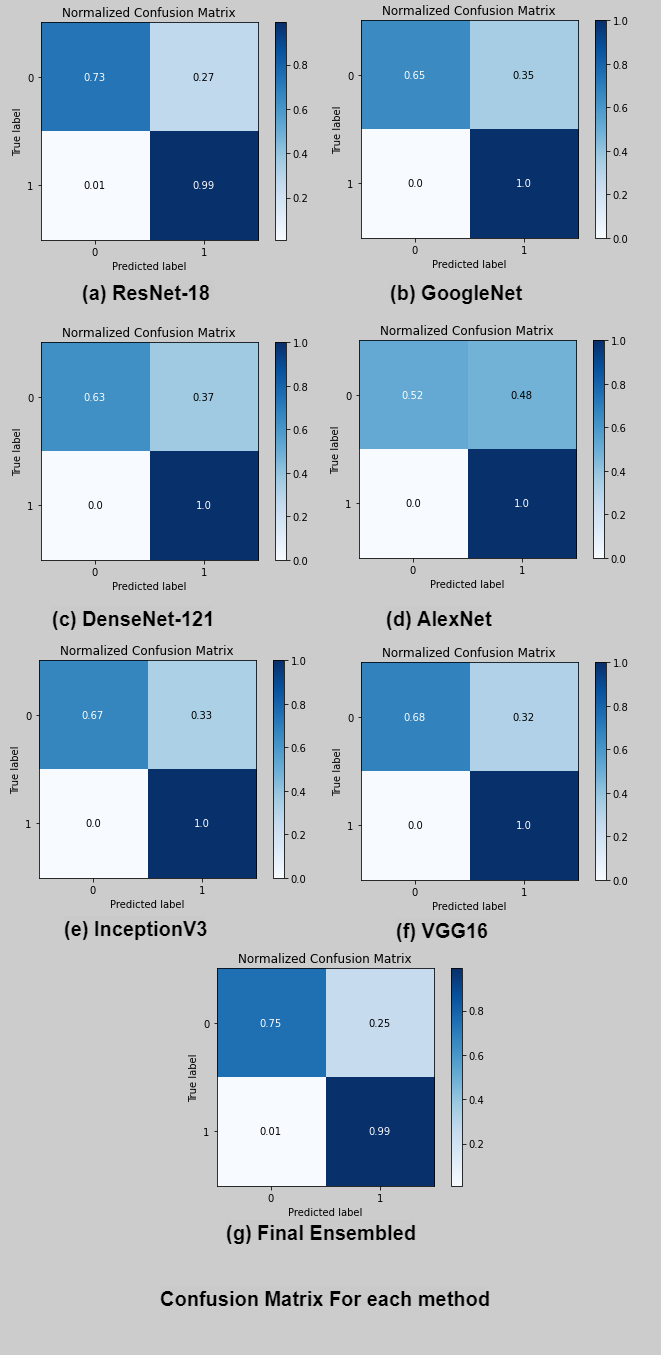
\includegraphics[width=0.5\textwidth, inner]{cm.png}
\caption{Confusion matrix for each learner and Ensemble}
\label{fig:cm}
\end{figure}
The accuracy rate gives a general proportion of the quantity of models right predictions. Nonetheless, if there is imbalance in dataset, a models high accuracy rate doesn't guarantee its capability to separate various classes equally. Specifically, medical imaging requires a model to be generalized to all the classes. Due to such scenarios, the "Recall" and "Precision" values give knowledge into the models performance. Positive label prediction of model are how much accurate is shown by Precision. This gives the proportion of the right predictions to the total number of predictions obtained by the model. Then again, "recall" gauges the level of ground true positives that the model accurately anticipated. These two assessment measurements survey whether the model can diminish the quantity of false negative and false positive predictions. "F1-Score" gives a harmony among recall and precision, thinking about both FNs and FPs. It punishes outrageous upsides of Recall and Prescision, every one of which is accomplished to the detriment of the other.



The Area Under the Curve (AUC) is ploted with values of True Positive and False Positive rates and measures the capacity of a classifier to recognize classes and is utilized as a rundown of the ROC curve where true positive shows the sample that belongs to positive class and being correctly predicted by the classifier and false positive indicates the sample being classify as positive class when in actual it belongs to negative class. The higher AUC shows better the exhibition of the model at recognizing the positive and negative classes. When AUC is 1, classsifier will predict both classes correctly and if it is 0, the classes predicted will be positive for negative and vice versa. The AUC curves for base learners and Ensemble method are shown in figure\ref{fig:auc} 

\begin{figure}[h]
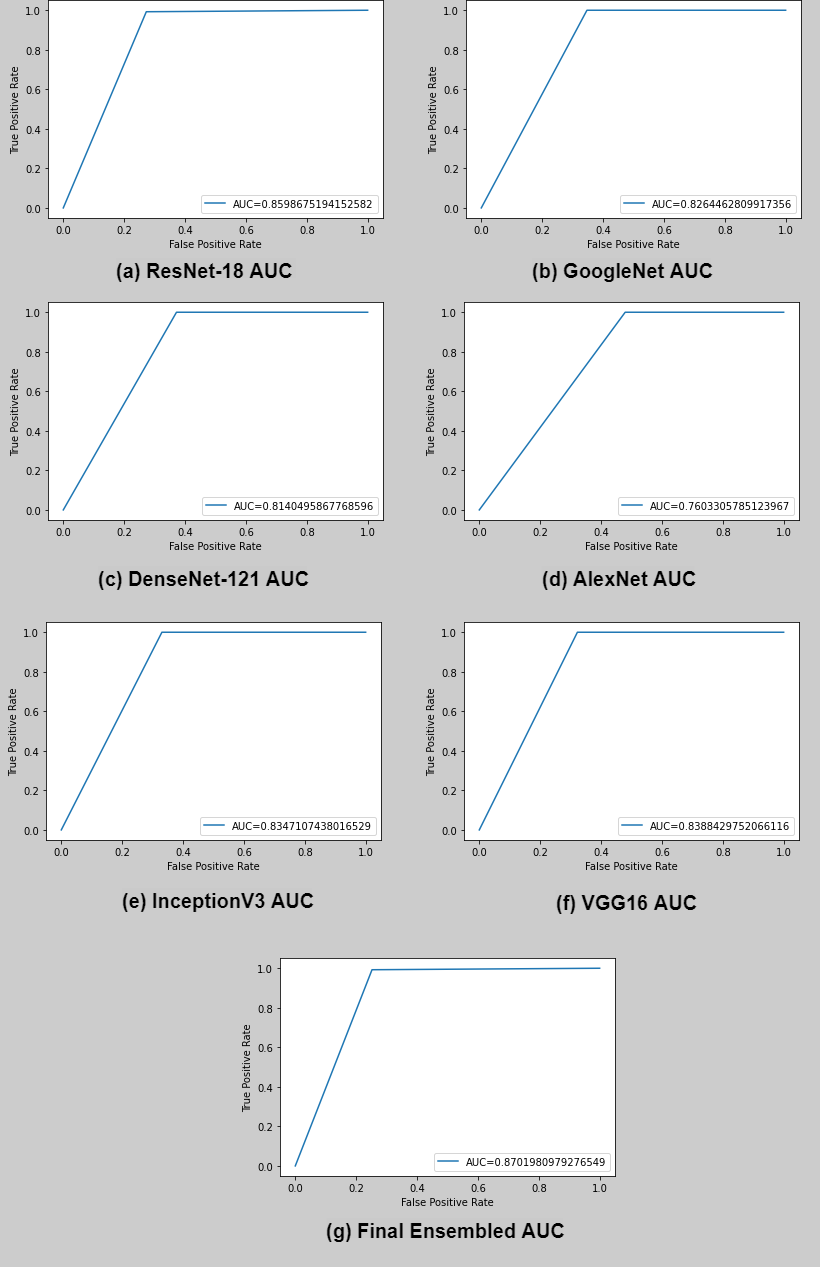
\includegraphics[width=0.5\textwidth, inner]{auc.png}
\caption{AUC for each learner and Ensemble}
\label{fig:auc}
\end{figure}
 The pretrained models were each trained on training dataset; Model training is learning the weights and bias from already labeled data prediction while accuracy and loss are measure of loos and accuracy on dataset where loss indicates how poor the model predicted on dataset while accuracy shows the percentage of correct predictions. Learning curves can be used to shown the learning changes in performance overtime, usually loss and accuracy should be decreased and increased respectively over epochs. where Training and validation accuracy and loss are shown in figure\ref{fig:accuracy} and figure\ref{fig:loss} respectively. 

\begin{figure}[h]
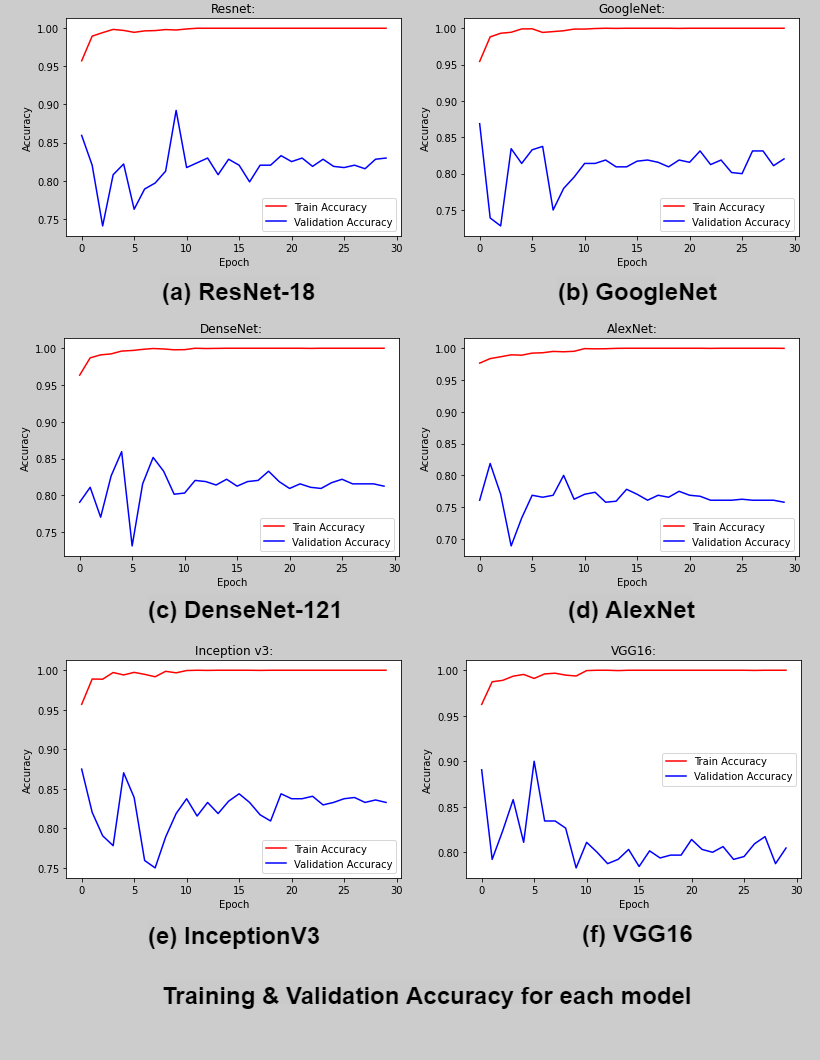
\includegraphics[width=0.5\textwidth, inner]{accuracy.png}
\caption{Training and Validation Accuracy}
\label{fig:accuracy}
\end{figure}

\begin{figure}[h]
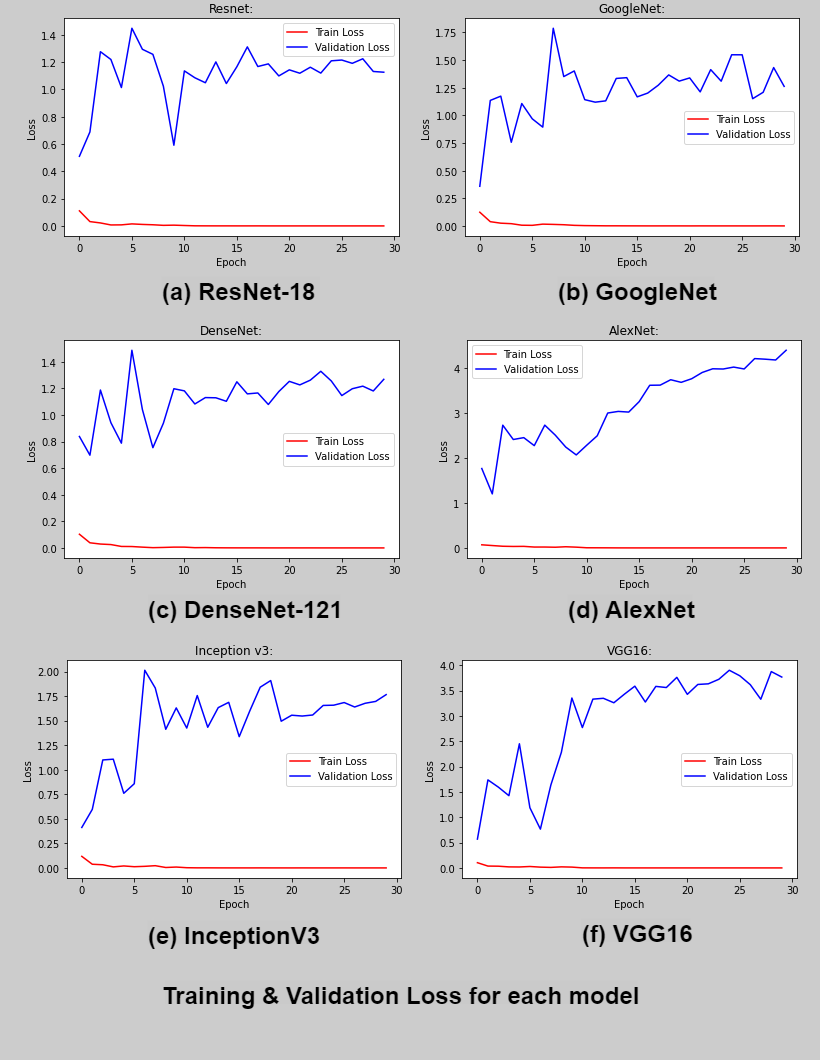
\includegraphics[width=0.5\textwidth, inner]{loss.png}
\caption{Training and Validation Loss}
\label{fig:loss}
\end{figure}




\section{Conclusion}
Detection or classification of medical images is very crucial as if gone wrong, it can produce complications. A computer-aided diagnosis system is proposed such that decision scores from different CNN base learners were used and then ensembled together such that evaluation metrics precision, AUC, recall, and f1-score and fed to hyperbolic tangent are used to assign a weighted average ensemble such that classifiers with high scores assigned with high priority. It produced Accuracy results of 90\%, Precision value of 91.06\%, Recall value of 90\%, and F1-Score is 89.66. It outperformed traditional CNN methods thus ensuring that the ensemble framework proposed captures needed information from base learners and its predictions are better than traditional methods. However, as seen in testing and validation loss curves, data must be balanced among classes else it will predict one class correctly but will produce wrong results on class with inferior data. Also, the computational cost needs to be under watched sue to use of multiple CNN classifiers..

\begin{thebibliography}{00}

\bibitem{b1} \emph{WHO Pneumonia. World Health Organization.}, 2019.
 \underline{https://www.who.int/news-room/fact-sheets/detail/pneumonia}

\bibitem{b2} Neuman MI, Lee EY, Bixby S, Diperna S, Hellinger J, Markowitz R, Servaes S, Monuteaux MC, Shah SS, \emph{Reliability of CXR for Pneumonia.} J. Hosp. Med 2012;4;294-298. doi:10.1002/jhm.955

\bibitem{b3}Williams, G.J., Macaskill, P., Kerr, M., Fitzgerald, D.A., Isaacs, D., Codarini, M., McCaskill, M., Prelog, K. and Craig, J.C. ``Variability and accuracy in interpretation of consolidation on chest radiography for diagnosing pneumonia in children under 5 years of age.'' \emph{Pediatr Pulmonol}, 2013

\bibitem{b4} Kermany D., Zhang K. & Goldbaum M, `` Labeled Optical Coherence Tomography (OCT) and Chest X-Ray Images for Classification'' 2018.

\bibitem{b5} Lal S., Rehman S., Shah J., Meraj T., Rauf H., Damaševičius R., ``Adversarial Attack and Defence through Adversarial Training and Feature Fusion for Diabetic Retinopathy Recognition,'' \emph{Sensors.}2021

\bibitem{b6} Rauf H., Lali M., Khan M., Kadry S., Alolaiyan H., Razaq A., et al, ``Time series forecasting of COVID-19 transmission in Asia Pacific countries using deep neural networks.'' \emph{Personal And Ubiquitous Computing}2021.

\bibitem{b7} Deng J., Dong W., Socher R., Li L., Li K. & Fei-Fei, L., ``Imagenet: A large-scale hierarchical image database.'' \emph{IEEE Conference On Computer Vision And Pattern Recognition.}2009

\bibitem{b8} Dalhoumi S., Dray G., Montmain J., Derosière, G. & Perrey S,''An adaptive accuracy-weighted ensemble for inter-subjects classification in brain-computer interfacing'' \emph{7th International IEEE/EMBS Conference On Neural Engineering (NER)}2015

\bibitem{b9} Albahli S., Rauf H., Algosaibi A. & Balas V, ''AI-driven deep CNN approach for multi-label pathology classification using chest X-Rays'' \emph{PeerJ Computer Science}, 2021.

\bibitem{b10} Rahman T., Chowdhury M., Khandakar A., Islam K., Islam K., Mahbub Z., et al, ``Transfer learning with deep convolutional neural network (CNN) for pneumonia detection using chest X-ray''  Applied Sciences. 10, 3233 (2020)

\bibitem{b11} Liang G. & Zheng L, ''A transfer learning method with deep residual network for pediatric pneumonia diagnosis'' \emph{Computer Methods And Programs In Biomedicine.}2020

\bibitem{b12} Ibrahim A., Ozsoz M., Serte S., Al-Turjman F. & Yakoi P, '' Pneumonia classification using deep learning from chest X-ray images during COVID-19'', 2021

\bibitem{b13} Zubair S, '' An Efficient Method to Predict Pneumonia from Chest X-Rays Using Deep Learning Approach.'' \emph{The Importance Of Health Informatics In Public Health During A Pandemic.} 2020

\bibitem{b14} Rajpurkar P., Irvin J., Zhu K., Yang B., Mehta H., Duan T., et al. & Others, ``Chexnet: Radiologist-level pneumonia detection on chest x-rays with deep learning'' \emph{ ArXiv Preprint ArXiv:1711.05225. (2017)}

\bibitem{b15} Albahli S., Rauf H., Arif M., Nafis M. & Algosaibi A, ``Identification of thoracic diseases by exploiting deep neural networks.'' \emph{Neural Networks.}, 5 pp. 6 (2021)

\bibitem{b16} Chandra T. & Verma K, ``Pneumonia detection on chest X-Ray using machine learning paradigm'' \emph{ Proceedings Of 3rd International Conference On Computer Vision And Image Processing,}pp. 21-33 (2020)

\bibitem{b17} Kuo K., Talley P., Huang C. & Cheng L, ''Predicting hospital-acquired pneumonia among schizophrenic patients: a machine learning approach'',2019

\bibitem{b18} Yue H., Yu Q., Liu C., Huang Y., Jiang Z., Shao C., et al. & Others, ``Machine learning-based CT radiomics method for predicting hospital stay in patients with pneumonia associated with SARS-CoV-2 infection: a multicenter study'', 2020

\bibitem{b19} Sharma H., Jain J., Bansal P. & Gupta S, ''Feature extraction and classification of chest x-ray images using cnn to detect pneumonia.''.\emph{2020 10th International Conference On Cloud Computing, Data Science & Engineering (Confluence)}

\bibitem{b20} Stephen O., Sain M., Maduh U. & Jeong D. ''An efficient deep learning approach to pneumonia classification in healthcare'' \emph{ Journal Of Healthcare Engineering. 2019}

\bibitem{b21} Janizek J., Erion G., DeGrave A. & Lee S, '' An adversarial approach for the robust classification of pneumonia from chest radiographs'', \emph{Proceedings Of The ACM Conference On Health, Inference, And Learning}. 2020

\bibitem{b22} Zhang J., Xie Y., Pang G., Liao Z., Verjans J., Li W., et al. & Others, ``Viral Pneumonia Screening on Chest X-rays Using Confidence-Aware Anomaly Detection'' \emph{ IEEE Transactions On Medical Imaging. (2020)}

\bibitem{b23} Tuncer T., Ozyurt F., Dogan S. & Subasi A. `` A novel Covid-19 and pneumonia classification method based on F-transform.'' \emph{Chemometrics And Intelligent Laboratory Systems.} 2021

\bibitem{b26} Pan I., Cadrin-Chênevert A. & Cheng P. ``Tackling the radiological society of north america pneumonia detection challenge'' 2019

\bibitem{b29} Kadry S., Nam Y., Rauf H., Rajinikanth V. & Lawal I, ``Automated Detection of Brain Abnormality using Deep-Learning-Scheme: A Study.''2021 Seventh International Conference On Bio Signals, Images, And Instrumentation (ICBSII). pp. 1-5 (2021)

\bibitem{b30} IEEE Criteria for Class IE Electric Systems, IEEE Standard 308, 1969.

\bibitem{b31} Kundu R., Basak H., Singh P., Ahmadian A., Ferrara M. & Sarkar R. ''Fuzzy rank-based fusion of CNN models using Gompertz function for screening COVID-19 CT-scans.'', 2021

\bibitem{b32} Manna A., Kundu R., Kaplun D., Sinitca A. & Sarkar R ``A fuzzy rank-based ensemble of CNN models for classification of cervical cytology.'' \emph{Scientific Reports.} 2021.

\bibitem{b33} Kundu R, Das R, Geem ZW, Han GT, Sarkar R. ``Pneumonia detection in chest X-ray images using an ensemble of deep learning models.'' \emph{PLOS ONE} 2021.

\end{thebibliography}

\EOD

\end{document}
